\documentclass{standalone}
\usepackage{tikz}
\usetikzlibrary{patterns, positioning}
\usepackage[sfdefault]{ClearSans} %% option 'sfdefault' activates Clear Sans as the default text font
\usepackage[T1]{fontenc}

\begin{document}
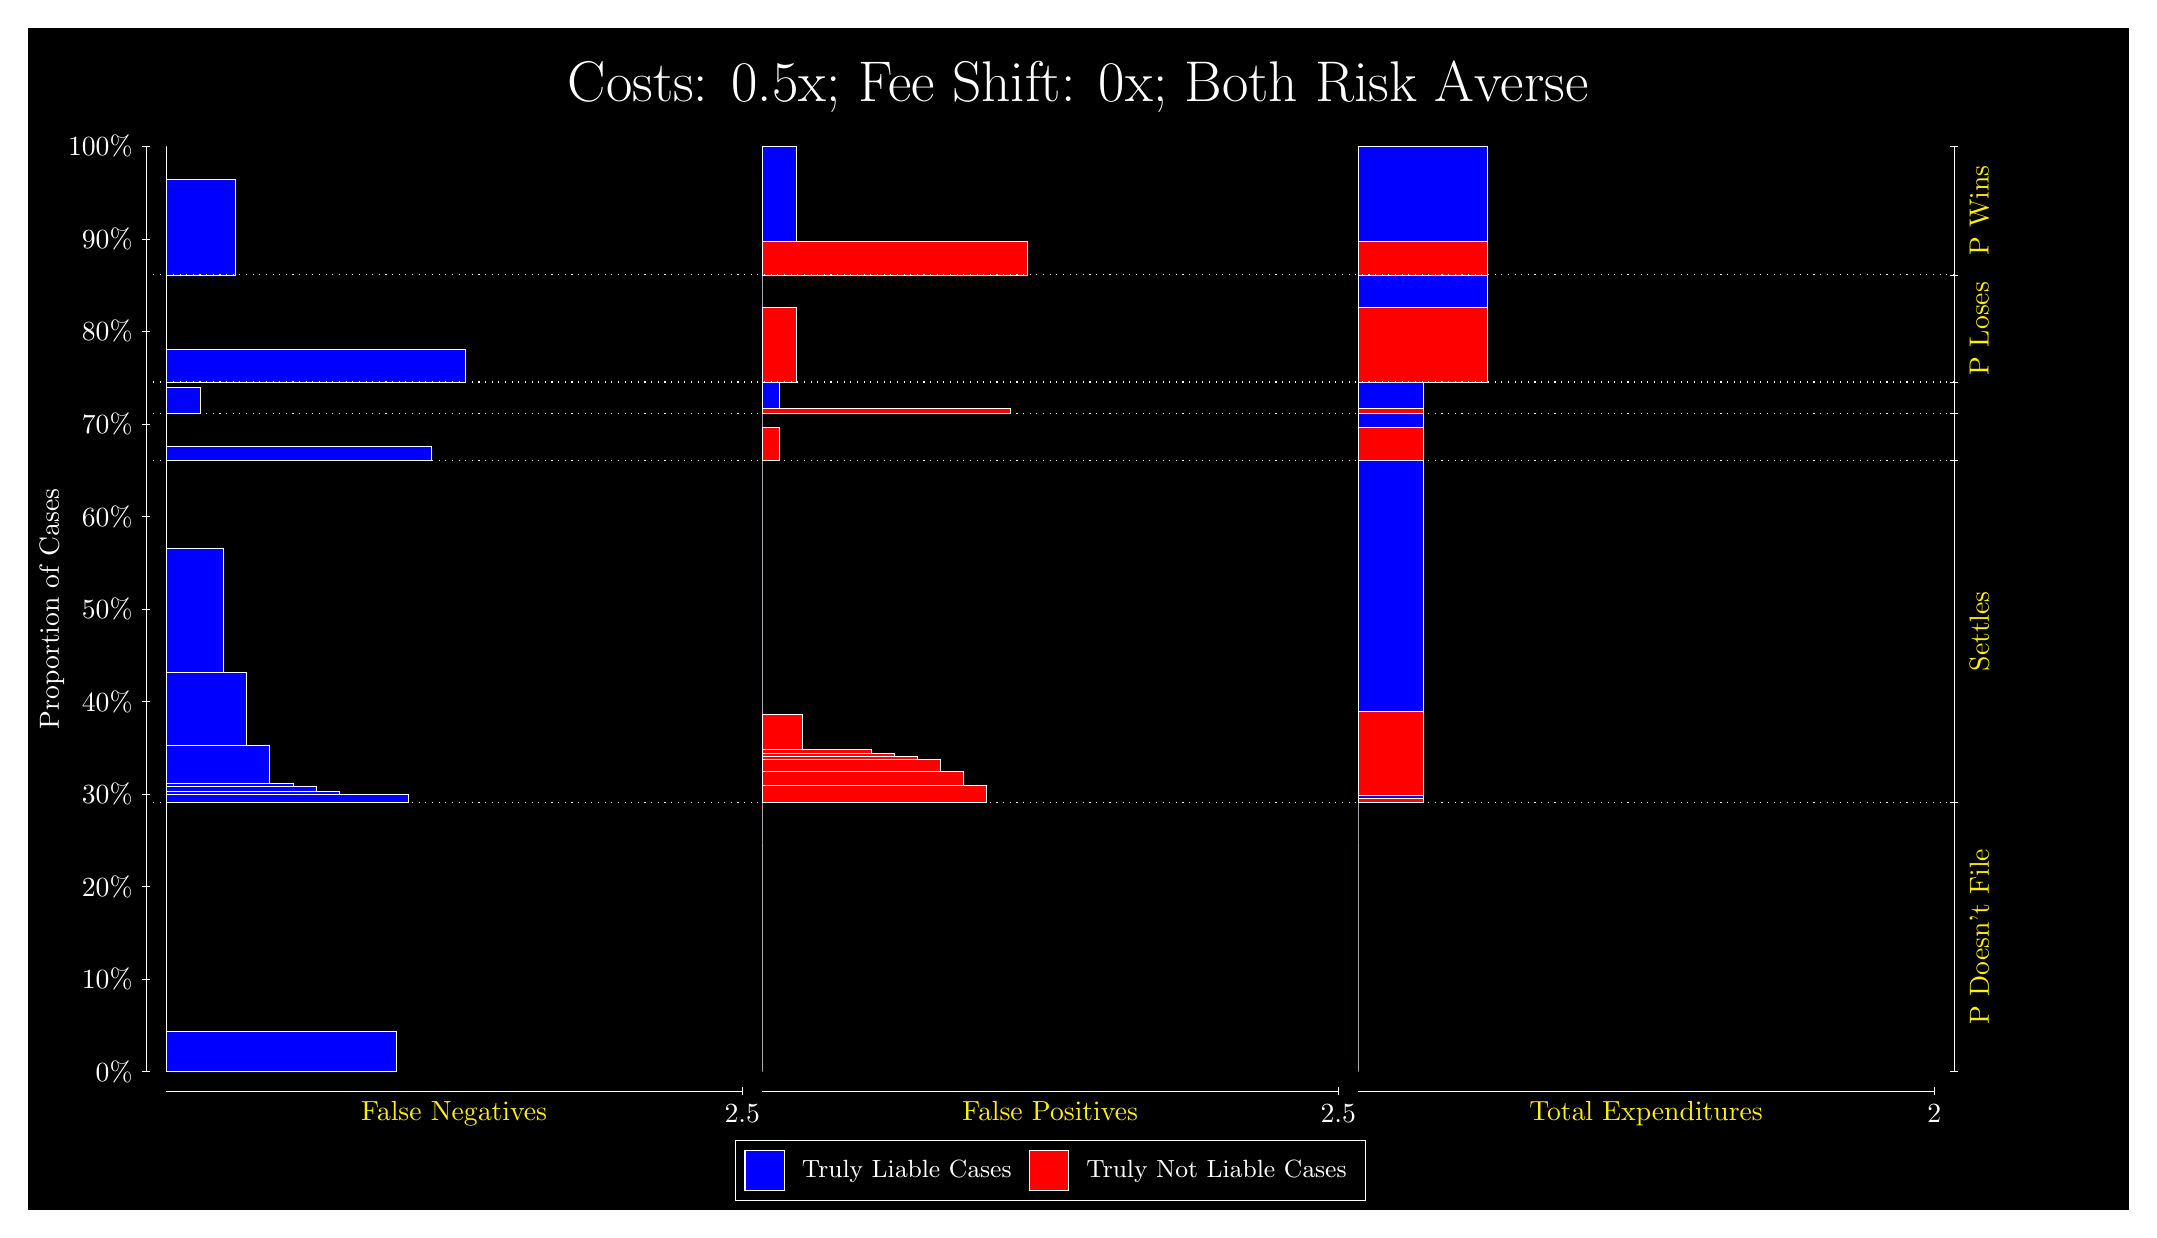
\begin{tikzpicture}
\draw[fill=black] (0,0) rectangle (26.667,15);
\draw[text=white] (0,13.5) rectangle (26.667,15) node[midway] {\huge Costs: 0.5x; Fee Shift: 0x; Both Risk Averse};
\draw[white, very thin] (1.5,1.75) -- (1.5,13.5);
\node[rotate=90, text=white, anchor=center] at (0.3, 7.625) {Proportion of Cases};
\draw[white, very thin] (1.45,1.75) -- (1.55,1.75);
\node[text=white, anchor=east] at (1.45, 1.75) {0\%};
\draw[white, very thin] (1.45,2.925) -- (1.55,2.925);
\node[text=white, anchor=east] at (1.45, 2.925) {10\%};
\draw[white, very thin] (1.45,4.1) -- (1.55,4.1);
\node[text=white, anchor=east] at (1.45, 4.1) {20\%};
\draw[white, very thin] (1.45,5.275) -- (1.55,5.275);
\node[text=white, anchor=east] at (1.45, 5.275) {30\%};
\draw[white, very thin] (1.45,6.45) -- (1.55,6.45);
\node[text=white, anchor=east] at (1.45, 6.45) {40\%};
\draw[white, very thin] (1.45,7.625) -- (1.55,7.625);
\node[text=white, anchor=east] at (1.45, 7.625) {50\%};
\draw[white, very thin] (1.45,8.8) -- (1.55,8.8);
\node[text=white, anchor=east] at (1.45, 8.8) {60\%};
\draw[white, very thin] (1.45,9.975) -- (1.55,9.975);
\node[text=white, anchor=east] at (1.45, 9.975) {70\%};
\draw[white, very thin] (1.45,11.15) -- (1.55,11.15);
\node[text=white, anchor=east] at (1.45, 11.15) {80\%};
\draw[white, very thin] (1.45,12.325) -- (1.55,12.325);
\node[text=white, anchor=east] at (1.45, 12.325) {90\%};
\draw[white, very thin] (1.45,13.5) -- (1.55,13.5);
\node[text=white, anchor=east] at (1.45, 13.5) {100\%};

\draw[white, very thin] (24.457,1.75) -- (24.457,13.5);
\draw[white, very thin] (24.407,1.75) -- (24.507,1.75);
\node[anchor=west] at (24.407, 1.75) {};
\draw[white, very thin] (24.407,5.1713) -- (24.507,5.1713);
\node[anchor=west] at (24.407, 5.1713) {};
\draw[white, very thin] (24.407,9.5142) -- (24.507,9.5142);
\node[anchor=west] at (24.407, 9.5142) {};
\draw[white, very thin] (24.407,10.111) -- (24.507,10.111);
\node[anchor=west] at (24.407, 10.111) {};
\draw[white, very thin] (24.407,10.507) -- (24.507,10.507);
\node[anchor=west] at (24.407, 10.507) {};
\draw[white, very thin] (24.407,11.868) -- (24.507,11.868);
\node[anchor=west] at (24.407, 11.868) {};
\draw[white, very thin] (24.407,13.5) -- (24.507,13.5);
\node[anchor=west] at (24.407, 13.5) {};

\draw[white, very thin, fill=blue] (1.75,1.75) rectangle (4.6775,2.265);
\draw[white, very thin, fill=red] (1.75,2.265) rectangle (1.75,5.1713);
\draw[white, very thin, fill=blue] (1.75,5.1713) rectangle (4.8239,5.2704);
\draw[white, very thin, fill=blue] (1.75,5.2704) rectangle (4.5312,5.2737);
\draw[white, very thin, fill=blue] (1.75,5.2737) rectangle (4.2384,5.277);
\draw[white, very thin, fill=blue] (1.75,5.277) rectangle (3.9457,5.3115);
\draw[white, very thin, fill=blue] (1.75,5.3115) rectangle (3.6529,5.3725);
\draw[white, very thin, fill=blue] (1.75,5.3725) rectangle (3.3602,5.4099);
\draw[white, very thin, fill=blue] (1.75,5.4099) rectangle (3.0674,5.89);
\draw[white, very thin, fill=blue] (1.75,5.89) rectangle (2.7746,6.8176);
\draw[white, very thin, fill=blue] (1.75,6.8176) rectangle (2.4819,8.4011);
\draw[white, very thin, fill=red] (1.75,8.4011) rectangle (1.75,9.5142);
\draw[white, very thin, fill=blue] (1.75,9.5142) rectangle (5.1167,9.6866);
\draw[white, very thin, fill=red] (1.75,9.6866) rectangle (1.75,10.111);
\draw[white, very thin, fill=blue] (1.75,10.111) rectangle (2.1891,10.438);
\draw[white, very thin, fill=red] (1.75,10.438) rectangle (1.75,10.507);
\draw[white, very thin, fill=blue] (1.75,10.507) rectangle (5.5558,10.925);
\draw[white, very thin, fill=red] (1.75,10.925) rectangle (1.75,11.868);
\draw[white, very thin, fill=blue] (1.75,11.868) rectangle (2.6283,13.08);
\draw[white, very thin, fill=red] (1.75,13.08) rectangle (1.75,13.5);
\draw[white, very thin, fill=red] (9.3189,1.75) rectangle (9.3189,4.6563);
\draw[white, very thin, fill=blue] (9.3189,4.6563) rectangle (9.3189,5.1713);
\draw[white, very thin, fill=red] (9.3189,5.1713) rectangle (12.173,5.3866);
\draw[white, very thin, fill=red] (9.3189,5.3866) rectangle (11.88,5.5574);
\draw[white, very thin, fill=red] (9.3189,5.5574) rectangle (11.588,5.7219);
\draw[white, very thin, fill=red] (9.3189,5.7219) rectangle (11.295,5.7483);
\draw[white, very thin, fill=red] (9.3189,5.7483) rectangle (11.002,5.7934);
\draw[white, very thin, fill=red] (9.3189,5.7934) rectangle (10.709,5.7939);
\draw[white, very thin, fill=red] (9.3189,5.7939) rectangle (10.709,5.8383);
\draw[white, very thin, fill=red] (9.3189,5.8383) rectangle (10.417,5.8414);
\draw[white, very thin, fill=red] (9.3189,5.8414) rectangle (10.124,5.8457);
\draw[white, very thin, fill=red] (9.3189,5.8457) rectangle (9.8312,6.2844);
\draw[white, very thin, fill=blue] (9.3189,6.2844) rectangle (9.3189,9.5142);
\draw[white, very thin, fill=red] (9.3189,9.5142) rectangle (9.5384,9.9382);
\draw[white, very thin, fill=blue] (9.3189,9.9382) rectangle (9.3189,10.111);
\draw[white, very thin, fill=red] (9.3189,10.111) rectangle (12.466,10.179);
\draw[white, very thin, fill=blue] (9.3189,10.179) rectangle (9.5384,10.507);
\draw[white, very thin, fill=red] (9.3189,10.507) rectangle (9.758,11.45);
\draw[white, very thin, fill=blue] (9.3189,11.45) rectangle (9.3189,11.868);
\draw[white, very thin, fill=red] (9.3189,11.868) rectangle (12.686,12.288);
\draw[white, very thin, fill=blue] (9.3189,12.288) rectangle (9.758,13.5);
\draw[white, very thin, fill=red] (16.888,1.75) rectangle (16.888,4.6563);
\draw[white, very thin, fill=blue] (16.888,4.6563) rectangle (16.888,5.1713);
\draw[white, very thin, fill=red] (16.888,5.1713) rectangle (17.711,5.1719);
\draw[white, very thin, fill=blue] (16.888,5.1719) rectangle (17.711,5.1728);
\draw[white, very thin, fill=red] (16.888,5.1728) rectangle (17.711,5.2245);
\draw[white, very thin, fill=blue] (16.888,5.2245) rectangle (17.711,5.2647);
\draw[white, very thin, fill=red] (16.888,5.2647) rectangle (17.711,6.3254);
\draw[white, very thin, fill=blue] (16.888,6.3254) rectangle (17.711,9.5142);
\draw[white, very thin, fill=red] (16.888,9.5142) rectangle (17.711,9.9382);
\draw[white, very thin, fill=blue] (16.888,9.9382) rectangle (17.711,10.111);
\draw[white, very thin, fill=red] (16.888,10.111) rectangle (17.711,10.179);
\draw[white, very thin, fill=blue] (16.888,10.179) rectangle (17.711,10.507);
\draw[white, very thin, fill=red] (16.888,10.507) rectangle (18.534,11.45);
\draw[white, very thin, fill=blue] (16.888,11.45) rectangle (18.534,11.868);
\draw[white, very thin, fill=red] (16.888,11.868) rectangle (18.534,12.288);
\draw[white, very thin, fill=blue] (16.888,12.288) rectangle (18.534,13.5);
\draw[white, dotted] (1.5,5.1713) -- (24.457,5.1713);
\draw[white, dotted] (1.5,9.5142) -- (24.457,9.5142);
\draw[white, dotted] (1.5,10.111) -- (24.457,10.111);
\draw[white, dotted] (1.5,10.507) -- (24.457,10.507);
\draw[white, dotted] (1.5,11.868) -- (24.457,11.868);
\draw[white, very thin] (1.75,1.5) -- (9.0689,1.5);
\node[text=yellow, anchor=north] at (5.4094, 1.5) {False Negatives};
\draw[white, very thin] (9.0689,1.45) -- (9.0689,1.55);
\node[text=white, anchor=north] at (9.0689, 1.45) {2.5};

\draw[white, very thin] (9.3189,1.5) -- (16.638,1.5);
\node[text=yellow, anchor=north] at (12.978, 1.5) {False Positives};
\draw[white, very thin] (16.638,1.45) -- (16.638,1.55);
\node[text=white, anchor=north] at (16.638, 1.45) {2.5};

\draw[white, very thin] (16.888,1.5) -- (24.207,1.5);
\node[text=yellow, anchor=north] at (20.547, 1.5) {Total Expenditures};
\draw[white, very thin] (24.207,1.45) -- (24.207,1.55);
\node[text=white, anchor=north] at (24.207, 1.45) {2};

\node[text=yellow, centered, rotate=90] at (24.777, 3.4606) {P Doesn't File};
\node[text=yellow, centered, rotate=90] at (24.777, 7.3427) {Settles};


\node[text=yellow, centered, rotate=90] at (24.777, 11.187) {P Loses};
\node[text=yellow, centered, rotate=90] at (24.777, 12.684) {P Wins};

\draw (12.978300999999998,1.5) node[draw=none] (baseCoordinate) {};
\begin{scope}[align=center]
        \matrix[scale=0.5, draw=white, below=0.5cm of baseCoordinate, nodes={draw}, column sep=0.1cm]{
            \node[rectangle, draw, minimum width=0.5cm, minimum height=0.5cm, fill=blue] {}; &
            \node[draw=none, font=\small, text=white] (B) {Truly Liable Cases}; &
            \node[rectangle, draw, minimum width=0.5cm, minimum height=0.5cm, fill=red] {}; &
            \node[draw=none, font=\small, text=white] (B) {Truly Not Liable Cases}; \\
            };
\end{scope}

\end{tikzpicture}
\end{document}